%% This is the dvc design chapter for my UBC PhD Dissertation
%% The parent document is called thesis.tex

\chapter{Digital volume correlation}
\label{ch:dvc}
As discussed in the introduction to this thesis, validation of computational data is key to its interpretation.
Finite element code is often used to predict the deformations of the cancellous bone -- a measure for which it has never been validated.
There are a number of \ac{fe} studies that are indicating that the cancellous bone compartment may play a critical role in hip fracture, but until the deformations measured in the cancellous bone can be validated, these results should be interpreted with a degree of scepticism.

Digital volume correlation (\acs{dvc}) is a technique similar to \acf{dic} which uses digital image tracking to determine the motion of a texture in two sequential images of the same thing under different loading conditions.
The tracking is done based on registration of subregions of the first image with the second image (Figure~\ref{fig:DVC_how}).
Once a number of subregions have been tracked, the relative displacement of each region can be used to calculate strain.
This strain value can then be compared to \ac{fe} calculated strain fields as a validation.

\begin{figure}
\centering
\includegraphics[width=0.7\linewidth]{./appendixDvc/figures/DVC_how}
\caption[Illustration of the \acs*{dvc} method]{\textbf{In \acs{dvc}, regions of the undeformed image are transformed and registered to a second image of the same object after deformation.} Graphic \textcopyright Seth Gilchrist, 2013.}
\label{fig:DVC_how}
\end{figure}

Similarly to \ac{fe}, this technique is computational in nature, but does not use any a prior knowledge of the potential deformations, making it an independent measurement technique.
While it may not be possible to conclude that it is a fully qualified measurement method (there remains no way to take objective measures of the occluded cancellous bone compartment), comparison with \ac{fe} using Bland-Altman plots would provide a source of verification~\citep{schlesinger_terminology_1979}.

\section{The \acs*{dvc} technique}
\label{sec:dvc_technique}
\acs{dvc} works by comparing two images on a subregion basis and computing the motion of each subregion between the images.
To acquire theses images, an object is imaged multiple times while undergoing loading.
The first image will be of the unloaded object, the second image will be at some finite load, and each successive image will be at incrementally higher load.
The images can then be compared to the first, unloaded image, or to the previously acquired image in order to determine the deformation between the two load levels.
The common terminology for the two images are the \textit{fixed} and \textit{floating} or \textit{moving} images.
The fixed image is used as the reference image and the floating image is registered to the fixed image.
In the present \ac{dvc} algorithm, the fixed image is the one from the higher load condition, and the floating image is the one from the lower load condition.

In order to register to images, there must be a semi-random image texture that allows for determination of a unique match between the two images.
Cancellous bone imaged using \ac{ct} is a good candidate because it contains a texture, which while being regular in nature, is unique at any given location.

The \ac{dvc} techniques described in this section were carried out in custom software programmed in \ac{cpp} and utilizing the \acf{vtk} and the \acf{itk}.
The source code can be found in \S\ref{sec:code_dvc}.

\section[Digital volume correlation design]{Design and implementation of a digital volume correlation algorithm}
\label{sec:dvc_implement}
On its face, the \ac{dvc} method is relatively simple.
The steps of the \ac{dvc} method are:
\begin{enumerate}
\label{lst:dvcMethod}
\item \label{dvc:imageUnloaded} \ac{ct} a bone in an unloaded state.
\item \label{dvc:imageLoaded} \ac{ct} the bone in a loaded state.
\item \label{dvc:readImages} Read in the loaded and unloaded images.
\item \label{dvc:globalReg} Globally register the two images to ensure overlap and good initial guess.
\item \label{dvc:subregion} Break the images into subregions. The fixed image subregions will be large, and the moving image subregions will be smaller.
\item \label{dvc:register} Register a moving subregion within the corresponding fixed subregion.
\item \label{dvc:errorDetect} Check for possible errors in the calculation and label regions for reanalysis.
\item \label{dvc:reRegister} Perform secondary registration on regions identified as erroneous.
\item \label{dvc:store} Store the translation data of the registration in a new image with a voxel located at the centre of the fixed subregion.
\item \label{dvc:differentiate} Spatially differentiate the translation data to obtain strain.
\end{enumerate}

The parameters used while performing these tasks are related to the methods of each task.
There are three main tasks being performed: imaging, subdividing and registration.
The decisions made about how each of these are performed influence the overall reliability, robustness and speed of the process.

\subsection{Imaging for \acs*{dvc}}
\label{sec:dvc_implement_imaging}
Imaging for \ac{dvc} can be done in multiple ways.
The only requirements are that it provide texture at a resolution sufficient to realize the texture.
Previous researchers who have used \ac{dvc}, or a variant of, have used \ac{mri}~\citep{benoit_3d_2009} and \ac{ct}~\citep{bay_texture_1995, bay_digital_1999, bay_measurement_1999, bay_methods_2008, hardisty_whole_2009, hardisty_image_2010, lenoir_volumetric_2007, roux_three-dimensional_2008, smith_digital_2002}.
\acs{ct} is the modality of choice as the machines are more readily available in the resolution ranges required, and they work on differences in density which makes imaging in materials like conglomerate rock possible~\citep{lenoir_volumetric_2007, bornert_discrete_2010}.

The general rule for the imaging portion is to acquire images at as high a resolution possible.
This is because the end result of the registration process, discussed in \S\ref{sec:dvc_implement_register}, is highly dependent on the outcome resolution.
That said, if the resolution is too fine, the image sizes become cumbersome, especially when imaging whole bones which can be many \acl{cm} in length.

\subsection{Subdividing images for \acs*{dvc}}
\label{sec:dvc_implement_subdivide}
Subdividing images into subregions for \ac{dvc} requires knowledge of your texture dimensions.
There are two dimensions to chose when subdividing an image: i) the size of each subregion, and ii) the spacing between subregions.

Since the registration relies on matching texture, each region must contain enough texture information to differentiate it from the surrounding image, and this is used to determine the size of each region.
In the case of \ac{dvc} the texture is the trabecular structure, so knowledge of aspects like \acl{tbsp} and \acl{tbth} allow for selection of this number.
For registration, the larger the subregions, the more accurate the registration due to the increased data volume.
However, in terms of strain measurement, smaller subregions are preferable as the registration steps will tend to return an average displacement over the region and larger regions lead to more averaging.
Additionally, if the regions become too large, holding them in memory while performing registration can be challenging.
In the presented method, both subregions are loaded into the computer's \acs{ram} in their entirety.
Modifying the code to stream only the sections currently under consideration could make the \ac{ram} requirements more manageable.

Due to a dearth of information regarding what an appropriate volume dimension is for \ac{dvc}, dimensions were taken from the \ac{dic} literature to justify the selection.
Researchers in \ac{dic} have determined that speckle size, subregion dimensions and pattern entropy all influence the outcome of the calculation~\citep{pan_study_2008, yaofeng_study_2007, lecompte_quality_2006}.
The most robust method for determination of subset size is subset entropy~\citep{yaofeng_study_2007} and the \ac{sssig}~\citep{pan_study_2008}, both of which are summations of gradients over the subregion.
Other researchers have shown that subregion size can be chosen based on the mean texture size~\citep{lecompte_quality_2006}, which in the case of \ac{dic} is a dot speckle.
The experiments on three different speckle patterns utilizing multiple subregions sizes showed that a region that was 2.3x to 4.3x the size of the texture was appropriate.
While using the gradient based measures would lead to the most robust subregion dimensions on a subregion-by-subregion basis (it would be evaluated dynamically during subdivision), a value based on the trabecular dimensions was desired to make implementation easy and intuitive.
For this reason, a selection of 3x \ac{tbsp} was selected.
This was used as it would ensure that at least two trabeculae were included in each direction, but kept the subregion size to a minimum.

\acused{DELTA}
\acused{delta}
\acused{x/dvc}
\acused{n/dvc}
\acused{eps}
\acused{l/dvc}
\acused{L/dvc}

Spacing of the subregions, along with the accuracy of the registration, influences the overall uncertainty of strain.
Equation~\ref{eq:dvc_strain1} gives the definition of engineering strain in a single dimension, where \ac{eps} is strain, \ac{DELTA}\textit{\ac{l/dvc}} is the change in length, and \textit{\ac{L/dvc}} is the original length.
Equation~\ref{eq:dvc_strain2} expands that definition to the average strain between two points, where \textit{\ac{x/dvc}}$_{\textit{\ac{n/dvc}}}$ is the original position at location \textit{\ac{n/dvc}}, and \ac{DELTA}\textit{\ac{x/dvc}}$_{\textit{\ac{n/dvc}}}$ is the change position at location \textit{\ac{n/dvc}}.
If we assume that we know the starting positions with absolute certainty, the uncertainty of the strain measure reduces to Equation~\ref{eq:dvc_strain3}, in which \ac{delta}(\ac{DELTA}\textit{\ac{x/dvc}}$_{\textit{\ac{n/dvc}}}$) is the uncertainty of the change in position at location \textit{\ac{n/dvc}}.
Calculating the partial derivatives, and substituting into Equation~\ref{eq:dvc_strain3} gives the strain uncertainty in terms of the position change uncertainty.
What we see is that the strain error is inversely related to the original distance between the measurement points (Equation~\ref{eq:dvc_strain5}), i.e., the larger the distance between the subregions, the lower the strain error, regardless of the registration error.
This also shows that the strain error is directly related to the registration, which is an intuitive result.
\vspace{-1EX}
\begin{eqnarray}
\varepsilon &=& \frac{\Delta\ell}{L} \label{eq:dvc_strain1} \\
			&=& \frac{\Delta x_2 - \Delta x_1}{x_2-x_1} \label{eq:dvc_strain2} \\
\delta\varepsilon &=& \delta(\Delta x_2) \cdot \frac{\partial\varepsilon}{\partial\Delta x_2} + \delta(\Delta x_1) \cdot \frac{\partial\varepsilon}{\partial\Delta x_1}\label{eq:dvc_strain3}\\
\frac{\partial\varepsilon}{\partial\Delta x_2} &=& \frac{1}{x_2-x_1}\label{eq:dvc_strain4}  = -\frac{\partial\varepsilon}{\partial\Delta x_1}\\
\therefore \delta\varepsilon &=& \frac{\delta(\Delta x_2) - \delta(\Delta x_1)}{x_2-x_1}\label{eq:dvc_strain5}
\end{eqnarray}

This shows that increasing the distance between subregions is advantageous from an accuracy perspective, however, increasing the spacing also has the unfortunate consequence of decreasing the resolution of the resulting strain field.
The upper bound on the spacing is therefore determined by desired accuracy and is normally determined using a set of validation experiments.
The lower bound can be set by considering the limits of the continuum assumption in the material that you are considering.
Work done to identify the limits of continuum theory~\citep{liu_minimum_2005} on inhomogeneous solids, as well as work in cancellous bone to determine the limits of continuity in \ac{fe} modelling~\citep{harrigan_limitations_1988} can provide insights that may guide us to a reasonable solution.
Theoretical work on cancellous bone suggests that continuum level analyses break down when \ac{fe} element sizes are less than 3-5 trabecular separations~\citep{harrigan_limitations_1988}.
The work in inhomogeneous solids suggests that a square volume with edges about 15x the crystal size in the solid gives consistent results~\citep{liu_minimum_2005}.
Based on the results from these experiments, it was determined that a region spacing between 5x and 15x \ac{tbsp} would be appropriate.
The final value would depend on the specimen, the variation of \ac{tbsp} across the specimen, and the smoothness of the results obtained at each spacing (e.g., erratic results would require reanalysis with larger separations).
In general, the first analysis of any specimen was conducted at 5x \ac{tbsp} and increased from there if results appeared erratic.

In summary, \ac{dvc} images were broken up in to square regions that were 3x \ac{tbsp} on a side, and separated by a minimum of 5x \ac{tbsp}.
These values could be increased if the strain fields appeared erratic, because increasing region size would tend to decrease the registration error, and increasing separation would decreases strain error according to Equation~\ref{eq:dvc_strain5}.

\subsection{Registration of image for \acs*{dvc}}
\label{sec:dvc_implement_register}
The registration of the subregions is the crux of the \ac{dvc} technique.
It has a number of sub-processes, each of which require decisions on the methods used to minimize error and computation time -- frequently competing interests.
The process (Figure~\ref{fig:Registration}) has two data structures, and four processes.
The data required for the process are the two images to be registered, in the case of the \ac{dvc} program these are the subregion images taken from the loaded and unloaded \ac{ct} images.
The processes are:
\begin{enumerate}
	\item Interpolator: interpolates the moving image pixel data into the grid of the fixed image.
	\item Metric: compares the interpolated moving image and the fixed image and provides a single value representing their agreement.
	\item Optimizer: computes the most likely position of the moving image that will result in good agreement with the fixed image.
	\item Transform: manipulates the grid of the moving image into a new space.
\end{enumerate}

\begin{figure}
\centering
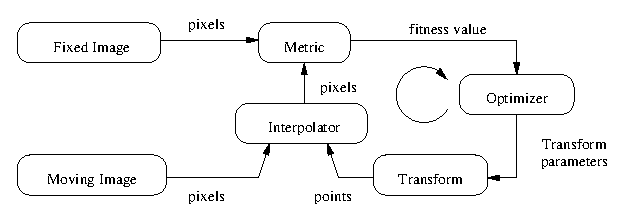
\includegraphics[width=\linewidth]{./appendixDvc/figures/SoftwareGuide-Art-RegistrationComponentsDiagram}
\caption[Image registration process]{\textbf{The image registration process operates in an iterative fashion.} Graphic from~\citet{ibanez_registrationcomponentsdiagram.fig_2003}, BSD-2 license, no permission required.}
\label{fig:Registration}
\end{figure}

The registration proceeds can be described as follows:
\begin{inparaenum}[(i)]
\item The two images are loaded into memory and the moving image is interpolated into the grid of the fixed image.
\item The metric computes the agreement between the two images and also in a neighbourhood of the current position.
This can be quite time consuming as the ``current position" is defined in terms of the transform parameters which can be numerous.
For a rigid transform there are six parameters (x, y, z translations and rotations), and for an affine transform in \acs{3d} there are 12 parameters.
\item The optimizer examines the metric value and local gradient and makes a decision on how to transform the moving image to better match the fixed image.
\item The moving image is modified based on the optimizer-determined transform and the interpolator interpolates the data of the transformed moving image into the grid of the fixed image.
\item Once the metric has reached a user-set criteria indicating a suitable match, the optimizer terminates the loop and returns the transform parameters.
\end{inparaenum}
Each of these processes can be done in a number of ways, and the relative strengths of each are discussed below.

\subsubsection{Interpolator}
\label{sec:dvc_implement_register_interpolator}
Interpolation is the method used to determine the value of the pixels between data points in a discrete dataset.
Images are a discrete representation of analogue information in which each pixel, or voxel as they are known in \ac{3d}, has a defined location and value.
The location of the voxel can typically be though of as accurate to the level of precision provided by the \ac{ct} machine used to generate the image.
The value of the voxel is an average value of the analogue data in the region around the location.
This \ac{3d} the region of averaging will be an ovoid, but for simplicity it is often thought of as being a cuboid~(Figure~\ref{fig:ImageData}).

\begin{figure}
\centering
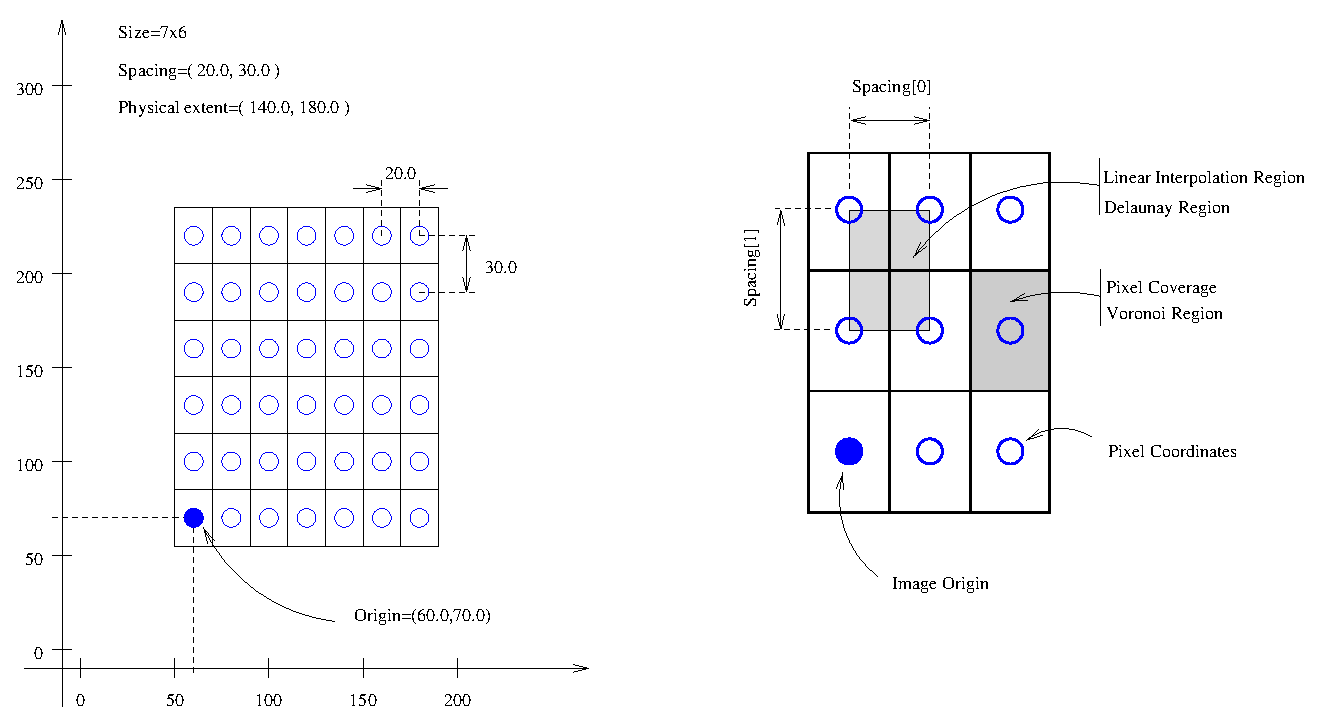
\includegraphics[width=\linewidth]{./appendixDvc/figures/SoftwareGuide-Art-ImageOriginAndSpacing}
\caption[Image data representation]{\textbf{Image data has point locations that are precise, and point values that are averages over the pixel Voronoi region. The Delaunay region is the space in which interpolation is necessary. In this example, the pixels of the image are not square, resulting in a rectangular Voronoi region. In \acs{3d} medical images, voxels are often defined with one dimension larger than the other two (the out-of-plane dimension).} Graphic from~\citet{ibanez_imageoriginandspacing.fig_2003}, BSD-2 license, no permission required.}
\label{fig:ImageData}
\end{figure}

When comparing two images, it is very unlikely that the grid of each image will line up exactly, especially after an arbitrary transform has been applied to one of the images.
This means that one would be comparing the data in the fixed image at a specific point, to the data in a moving image Delaunay region.
In order to perform the comparison, one must interpolate the value of the moving image in the Delaunay region.

The typical image interpolation techniques are (Figure~\ref{fig:Interpolations}):
\begin{inparaenum}[(i)]
\item  nearest neighbour, in which locations in the pixel's Voronoi region all a take the value of the pixel;
\item linear, in which a linear function is used to determine the value in the Delaunay region; and
\item \ac{bspline}, in which splines of order $\geq2$ are constructed and used to determine the value un the Delaunay region.
\end{inparaenum}

\begin{figure}
\centering
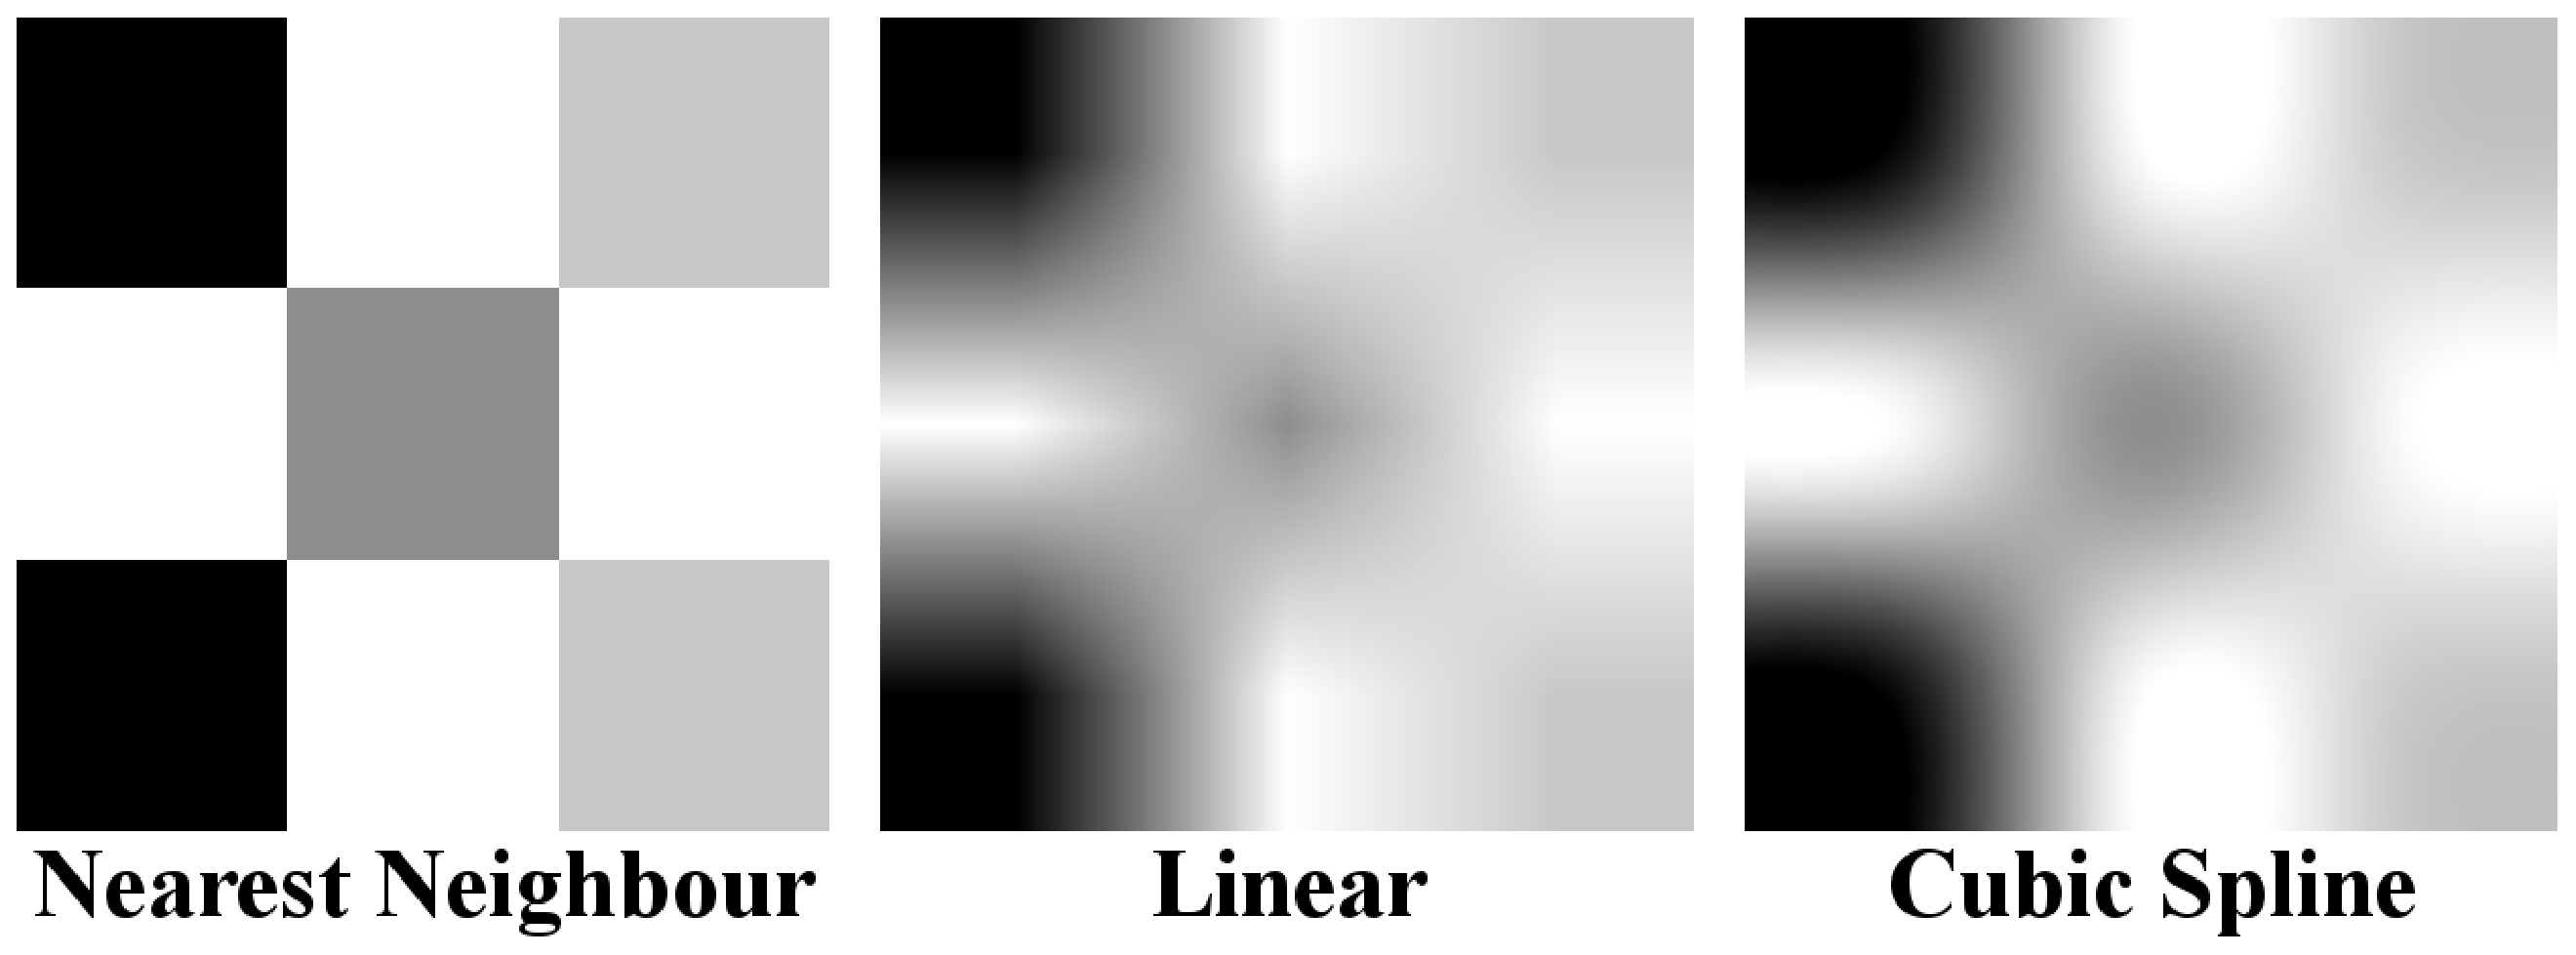
\includegraphics[width=\linewidth]{./appendixDvc/figures/Interpolations}
\caption[Interpolation of image data]{\textbf{Image data interpolated using nearest neighbour (left), linear (middle) and cubic \acs{bspline} (right) interpolation. It can be seen that linear and cubic spline give similar results.} Graphic \copyright Seth Gilchrist 2013.}
\label{fig:Interpolations}
\end{figure}

Nearest neighbour interpolation is used in image registration when aligning a label map to an image or another label map.
Interpolation of a label map has no meaning, e.g., if one has a label map of the cortical bone, cancellous bone and bone marrow, there is no meaning to interpolating between the them, pixels are either one or the other, not a mixture.
This type of interpolation is rarely used when interpolating image data, and is not used in the \ac{dvc} algorithm described here.
Linear interpolation is frequently used with image data because it gives reasonable results and is computationally inexpensive and fast.
\ac{bspline} interpolation is used when increased accuracy is needed, with the degree of computation being determined by the order of the spline used.
Investigators who have researched higher order interpolation routines~\citep{schreier_systematic_2000} have shown that for grey scale images (as opposed to binary images) a fourth order \ac{bspline} provides significantly lower error (up to 1/5$^{th}$) than a third order \ac{bspline}.

Testing of the \ac{dvc} algorithm using both quintic \ac{bspline} and linear interpolators showed that at small strain values there is an advantage to the \ac{bspline} interpolators (Figure~\ref{fig:CompareInterpolator}).
When a test image was synthetically strained to 1.6\% strain (as described in \S\ref{sec:dvc_results_validation}) the \ac{bspline} interpolator had a median error of approximately half that of the linear interpolator (0.0255 and 0.0488~voxels, respectively).
This advantage diminished when strains were larger, with the \ac{bspline} interpolator showing only an 8\% improvement when a maximum strain of 10\% was applied (0.2489 and 0.2708~voxels for the \ac{bspline} and linear interpolators, respectively).

\begin{figure}
\centering
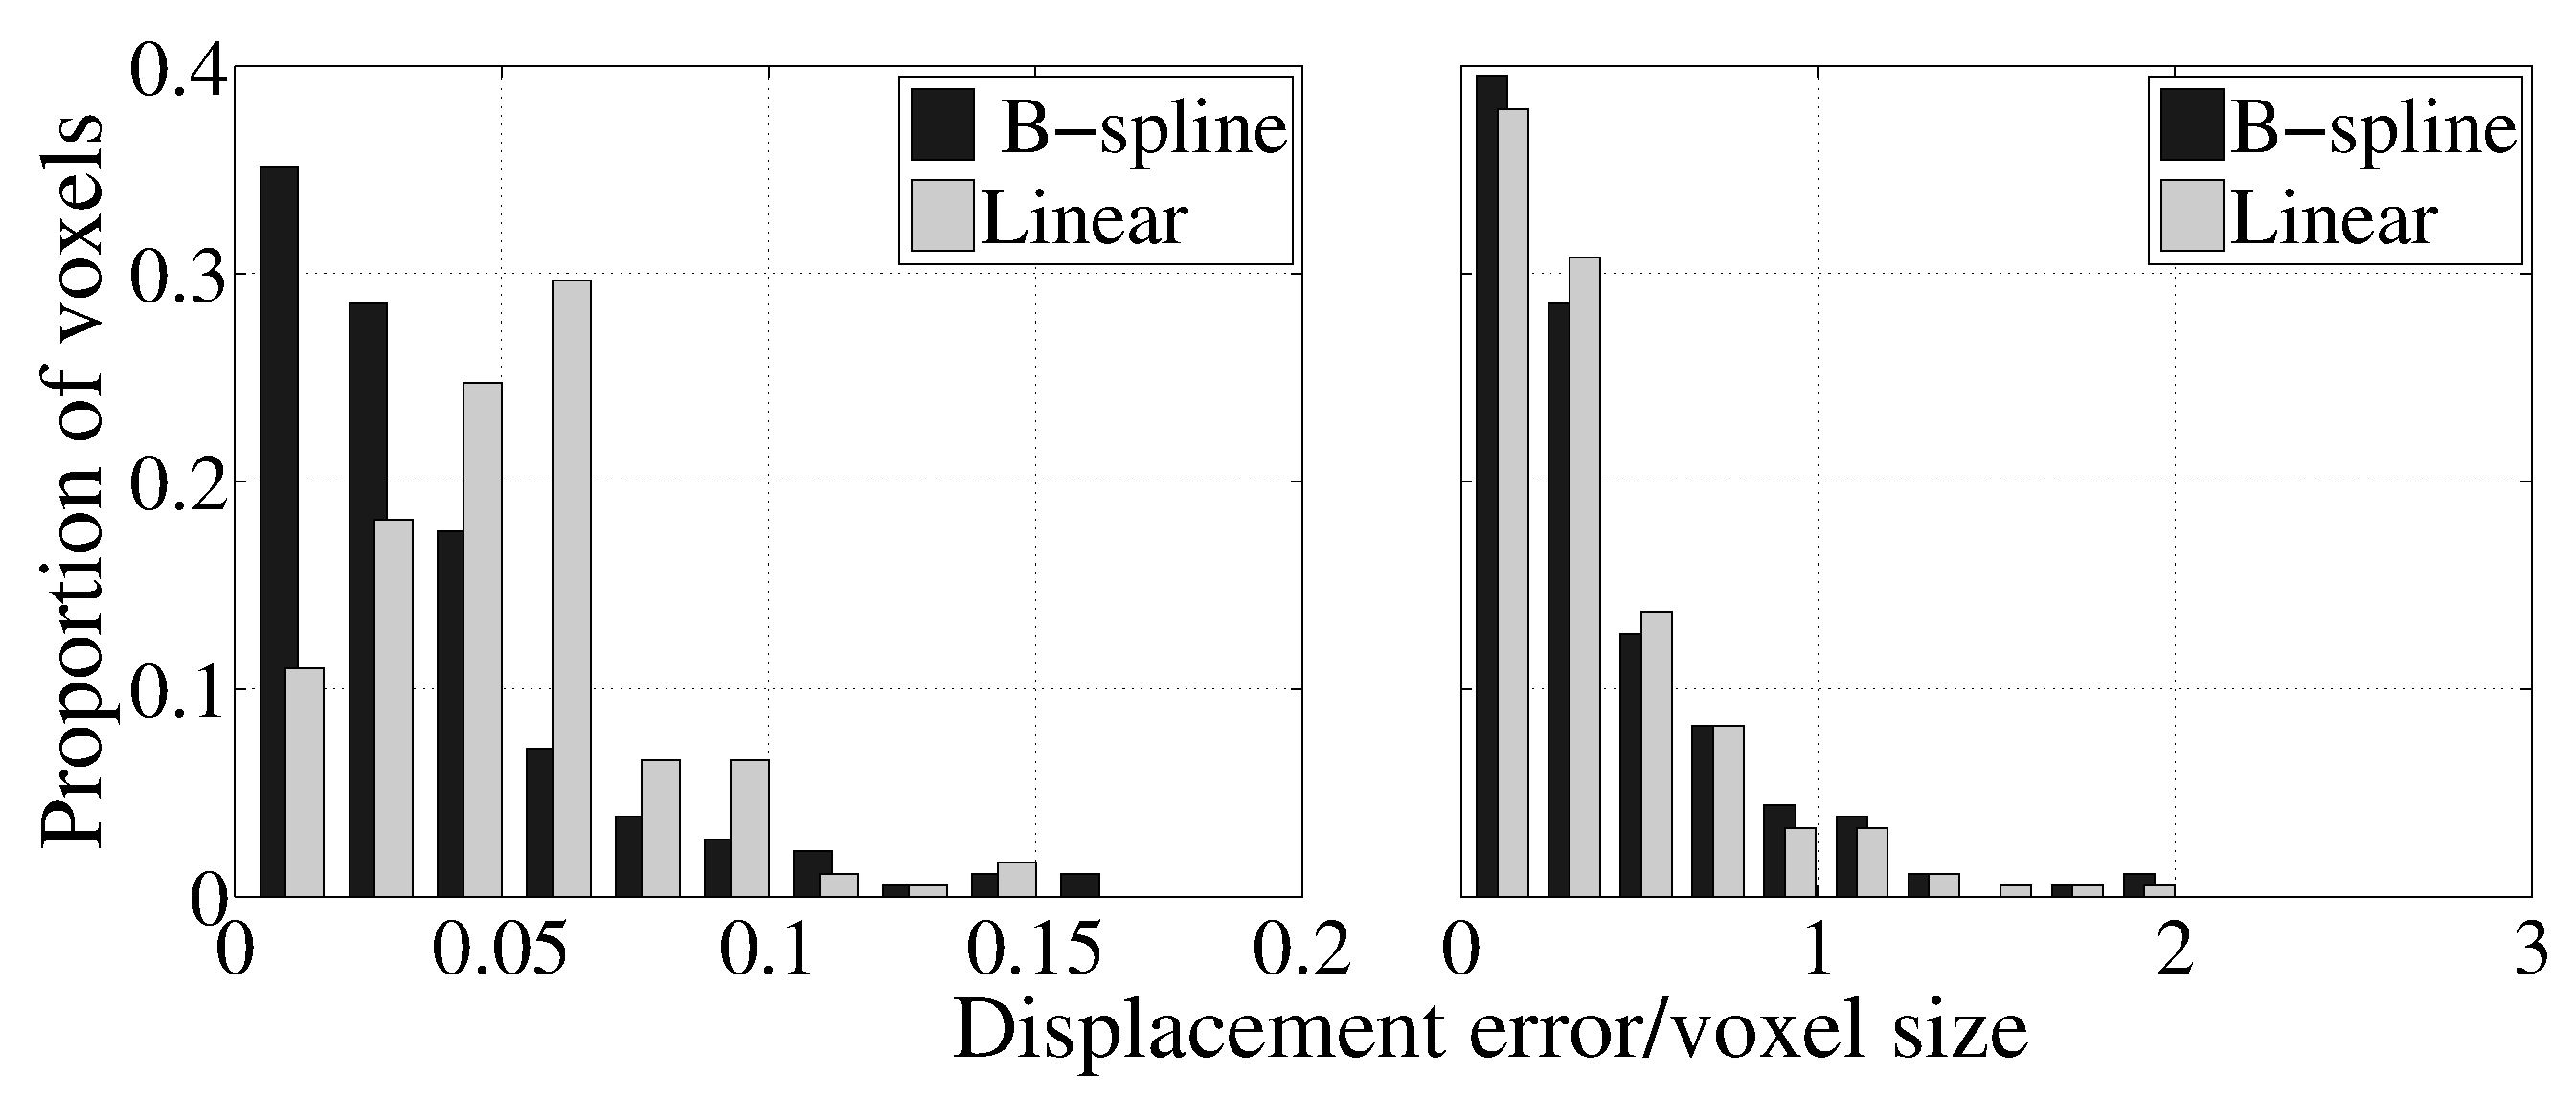
\includegraphics[width=\linewidth]{./appendixDvc/figures/CompareInterpolator}
\caption[Interpolator comparison]{\textbf{Comparison of linear and 4\textsuperscript{th} order \acs*{bspline} interpolation. When a synthetic strain with a maximum value of 1.6\%~\acs*{eps} was applied to an image, the \acs*{bspline} interpolator showed a clear advantage (left). This was not true when a synthetic strain with a maximum value of 10\%~\acs*{eps} was applied (right). Transformations were performed using affine transforms for this test.} Graphic \copyright Seth Gilchrist 2013.}
\label{fig:CompareInterpolator}
\end{figure}

The \ac{dvc} algorithm uses both linear and quintic \ac{bspline} interpolation.
In the global registration (Item~\ref{dvc:globalReg} on page~\pageref{dvc:globalReg}) linear interpolation is used.
This step is meant to give a good approximate starting position for the subregion registrations.
It operates on a large data set so needs to be fast and require little memory, making linear interpolation a good candidate.
During the registration of the subregions, the increased accuracy of the quintic \acp{bspline} is worth the computational cost to ensure accurate strain output.

\subsubsection{Metric}
\label{sec:dvc_implement_register_metric}
The metric is the most computationally expensive part of the registration.
That said, the performance of the metric directly affects the results of the registration, and the number of iterations required by the optimizer to reach the best match.
Metrics are either correlation or sum-squared difference functions, both of which share many fundamental characteristics and are closely related~\citep{tong_evaluation_2005}.

In order to reduce the computational expense of the process, we can take advantage of certain aspects of the \ac{hrpqct} imaging technique.
The most notable of these aspects is that image parameters such as lighting intensity are stable over time and between images.
This fact means that normalization of the images is not required, greatly reducing the computational cost~\citep{pan_two-dimensional_2009}.

For this reason, the non-normalized, sum-squared difference metric was used in the current \ac{dvc} technique.

\subsubsection{Transform}
\label{sec:dvc_implement_register_transform}
The transform is used to manipulate the moving image subregion such that it resembles the fixed image, making it possible to find a suitable match.
There are a number of different kinds of transforms with varying levels of complexity and varying numbers of parameters to characterize the deformation~(Table~\ref{tab:transforms}).

\begin{table}
\caption[Spacial transformations]{\textbf{Different \acs*{dic} transformations and their number of parameters in \acs*{3d}}~\citep{ibanez_itk_2003}.}
\label{tab:transforms}
\begin{tabularx}{\textwidth}{l X}
\toprule
	Rigid body & Six parameters: three translations and three rotations.\\
	Euler transform & Seven parameters: three translations, three rotations and a scaling. \\
	Affine & 12 parameters: nine for shear, rotation and scaling, and three for translations.\\
	\ac{bspline} deformable & Many parameters that describe and arbitrary warping of the image space. \\
\bottomrule
\end{tabularx}
\end{table}

Each of these transforms can describe different kinds and degrees of deformation.
The simplest of them is the Euler rigid body transform which describes only translations and rotations and therefore cannot account for actual changes in shape.
The affine transform is very versatile and is used in many image processing algorithms.
It has 12 parameters and is able to describe scaling, shear, translation and rotation in each of the three dimensions independently, it allows for significantly more deformation, with only five more parameters than the Euler transform.

Because the number transform parameters dictate the number of calculations that must be made by the metric when evaluating the gradient surrounding the current point, it is computationally advantageous to minimize the number of parameters.
In \ac{dic} the selection of the transform is often termed the shape-function selection~\citep{pan_two-dimensional_2009, lu_deformation_2000, schreier_systematic_2002}.
In order to be accurate, the deformation allowed for each subregion must be able to capture the change in shape of that subregion.
For small strains and small subregions, one can assume that the deformation across the region is linear, bur for larger strains and larger regions this assumption begins to break down.
For subfailure strain levels, first order shape functions have been shown to be as effective as higher order functions in sub-pixel registration~\citep{bing_performance_2006}.

For the current \ac{dvc} algorithm Euler and affine transforms were considered the best two candidates.
Tests performed using synthetically strained images (described in \S\ref{sec:dvc_results_validation}) were conducted using linear interpolation and changing the transformation between affine and Euler (Figure~\ref{fig:CompareTransforms}).
When a linear strain with a maximum value of 1.6\% was applied, the median displacement error measured by the affine and Euler transforms differed by 2.2\% (0.0474 and 0.0485~voxels for affine and Euler, respectively).
When the deformation was increased such that the maximum strain was 10\% the affine transform was 3.7\% better than the Euler transform (0.2708 and 0.2808~voxels for affine and Euler, respectively).
Even thought he difference in measured displacement errors was low in both cases, affine transformations showed a consistent reduction in error across all strain values.

\begin{figure}
\centering
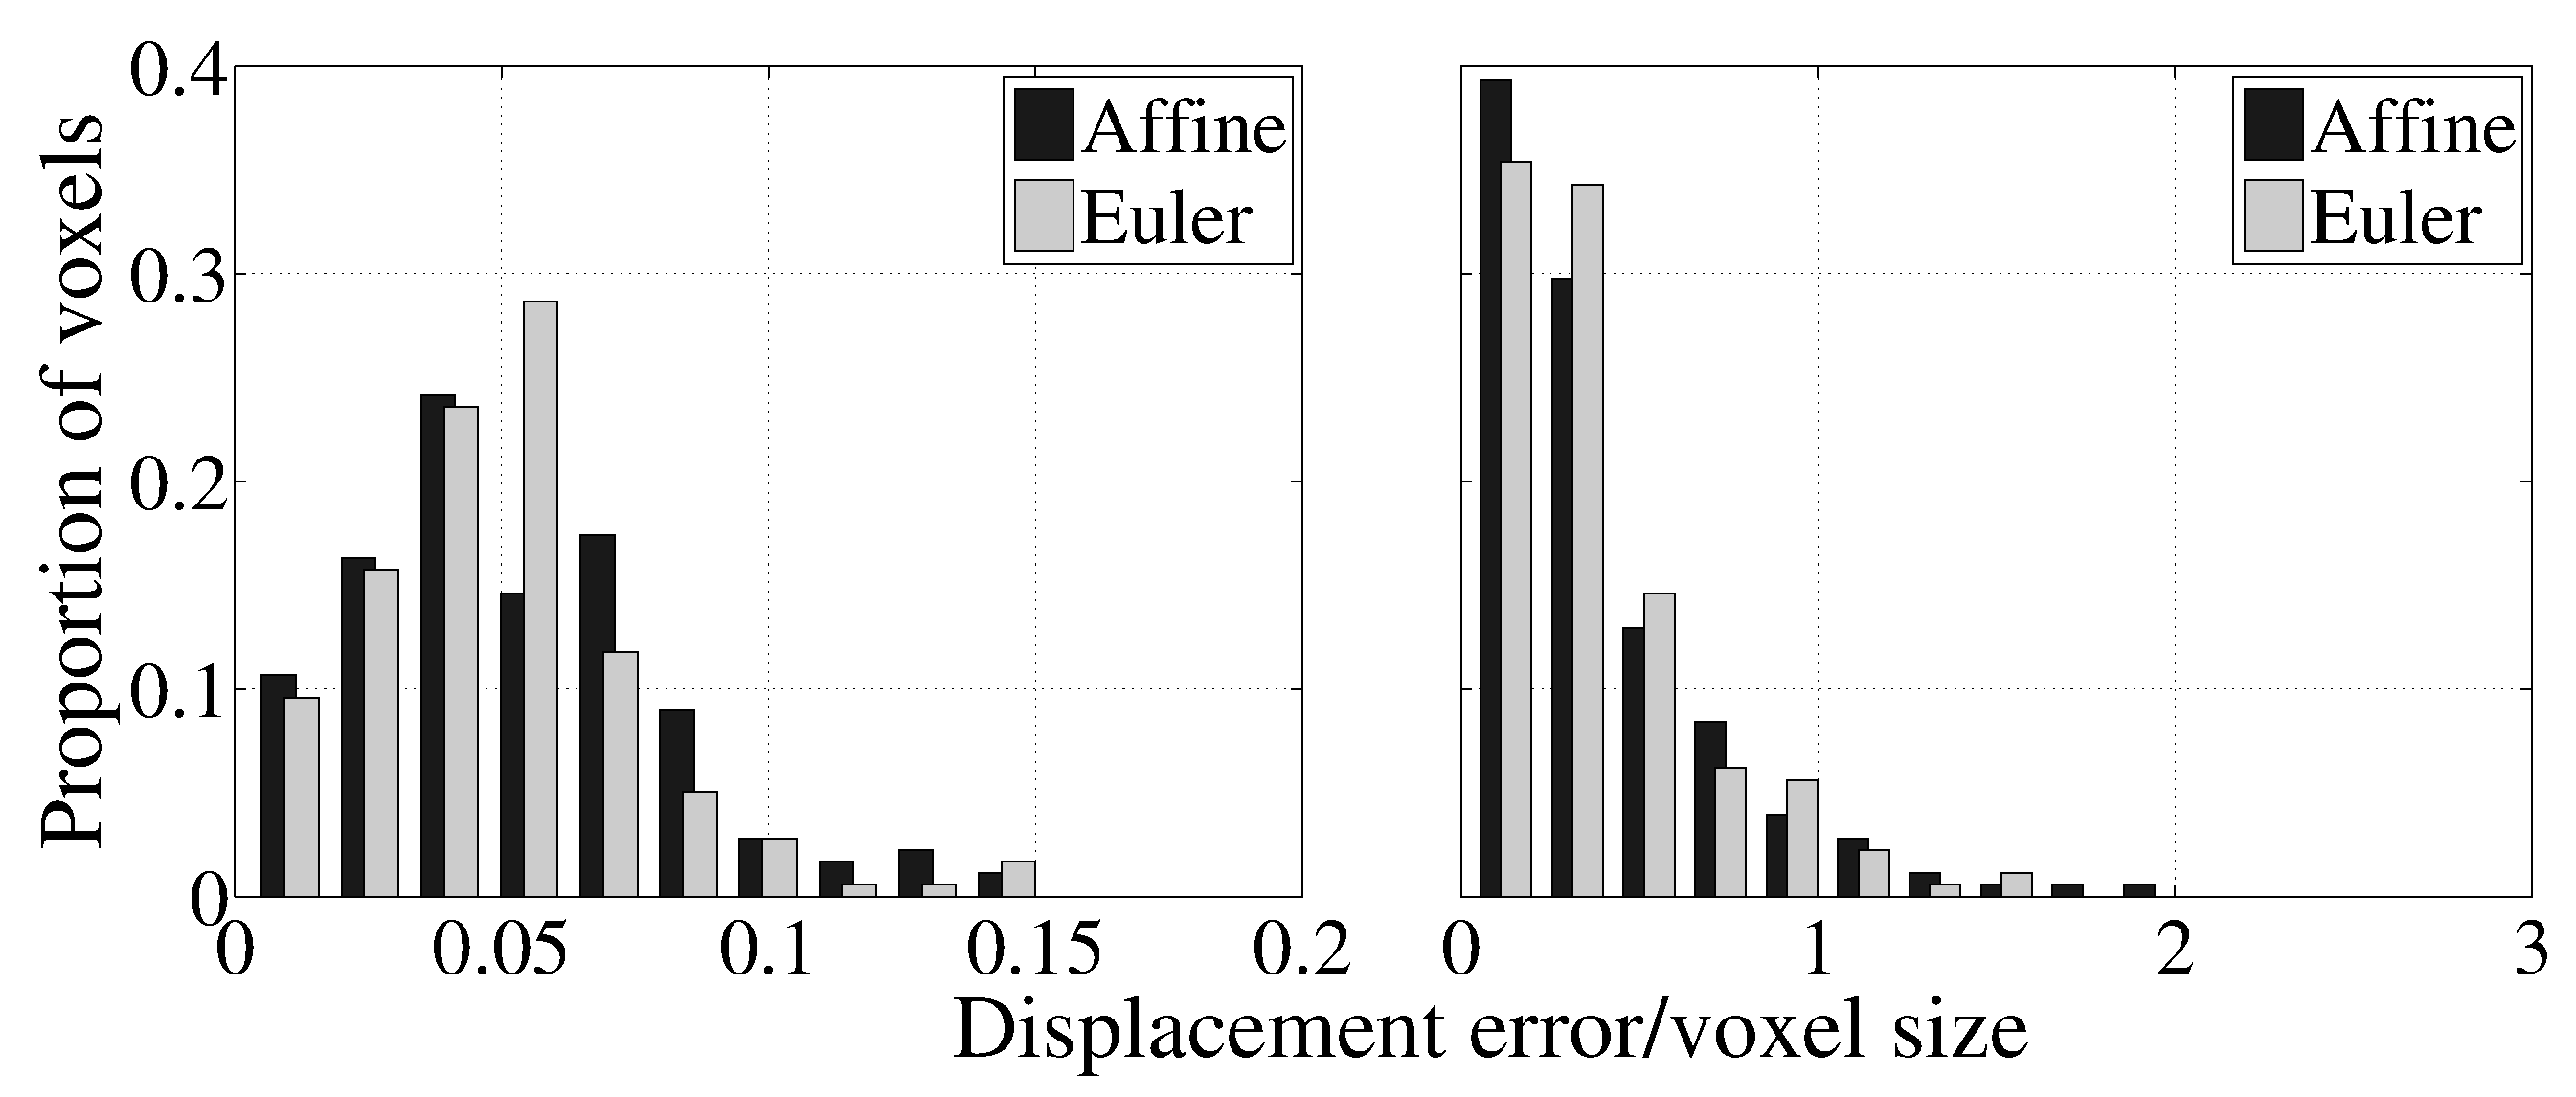
\includegraphics[width=\linewidth]{./appendixDvc/figures/CompareTransforms}
\caption[Transformation comparisons]{\textbf{Comparison of affine and Euler transformations. When a synthetic strain with a maximum value of 1.6\%~\acs*{eps} was applied to an image, the affine transform was seen to be moderately better (left). The comparison improved for the affine transform when a synthetic strain with a maximum value of 10\%~\acs*{eps} was applied (right). Transformations were performed using linear interpolations for this test.} Graphic \copyright Seth Gilchrist 2013.}
\label{fig:CompareTransforms}
\end{figure}

The \ac{dvc} algorithm described here was designed to use two different transforms.
An initial, global alignment of the two images is performed using a Euler rigid body transform.
This ensures that if the two images were separated in space due to placement in the \ac{ct} scanner, they are first roughly aligned so that they are fully overlapping.
The subregions are then mapped using affine transforms.
The decision to use the affine transform was made because the consistent improvement in displacement measurement across all strains would improve the overall results of the method.


\subsubsection{Optimizer}
\label{sec:dvc_implement_register_optimizer}
The optimizer makes decisions on how to deform the moving image such that it will correlate well with the fixed image.
Since registration is performed in real-world coordinates (rather than pixel-space), there are an infinite number of different possible solution locations.
This means that not all possible solutions, or even probable ones, can be tested in a reasonable time span, therefore a method to find the solution with the minimum number of iterations must be used.
This is the job of the optimizer.

Most classical optimizers work using the gradient of the metric field.
The metric provides a single value describing the agreement between the two images at a given transformation location.
The optimizer evaluates the metric in a neighbourhood around the current location and follows the gradient of the metric to either the maximum (in the case of correlation coefficient metrics) or the minimum (for sum-square difference metrics).

Newtonian optimizers have been shown to work well for \ac{dic} methods~\citep{bing_performance_2006}, however their assumption of a quadratic optimization problem can lead to a small radius of convergence.
Gradient descent methods are know to be robust, with a radius of convergence that can be tailored by selecting an appropriate initial step size.
That said, gradient descent optimizers are known to be inefficient, suffering from the ``ping-pong" effect where the optimizer will use ever smaller steps as one approaches the optimal solution~\citep{meza_steepest_2010}.
One way to help with this issue is to use a regular step, gradient descent optimizer which uses one step size until the sign of the gradient reverses, at which time it reduces the step size by a set relaxation factor and continues.
In this way, the step size is not determined by the magnitude of the gradient, but by the passing of the minimum, reducing the number of steps to convergence.

Previous researchers have examined the accuracy of different optimizers for \ac{dic} and found that while Newtonian methods gave the best results, there was a significant computational penalty for using them~\citep{bing_performance_2006}.
In fact, the Newtonian method took two orders of magnitude longer to solve than the gradient based method, even with the known inefficiency of the gradient methods.

To allow for the largest radius of convergence and highest speed, a regular step, gradient descent algorithm was used for the current \ac{dvc} algorithm.

\subsection{Error analysis}
\label{sec:dvc_implement_error}
The error analysis routine for the \ac{dvc} was used to detect and reanalyse subregion registrations that were determined to be likely erroneous.
The search for erroneous registrations was based on parametric statistics of the region under consideration and the connected analysis regions.
The results image was iterated through and for each region the average and standard deviation of the connected neighbours of the displacements in the \textit{x, y} and \textit{z} directions were calculated.
The tolerance for an erroneous result is set by the user at the start of the analysis in number of standard deviations from the connected neighbour mean.
For example, if point \textit{n} has a \textit{z}-displacement of 0.51~mm and the average and standard deviation of the \textit{z}-displacement for \textit{n}'s neighbours are .48~mm and .02~mm, respectively, this region would be reanalysed if the user set a tolerance of one standard deviation, but not if two standard deviations were used.
If a region is flagged for reanalysis, an initial guess of its solution was set as the average of the valid neighbours displacements.

\subsection{Data storage}
\label{sec:dvc_implementation_storage}
The data for the \ac{dvc} algorithm is stored in a \acl{fe} style mesh.
Initial versions of the algorithm used a regular grid (similar to an image), but this method required too many analyses for large datasets and also didn't have the flexibility to represent complex shapes while maintaining proper subregion spacing.
Other advantages of the \ac{fe} mesh is that algorithms for calculating the derivatives (i.e., strains) have been developed and did not have to be implemented from scratch.
The open-source mesh generator Gmsh (\url{http://geuz.org/gmsh/}) was used to generate the meshes and the \ac{dvc} algorithm could read in either a Gmsh mesh, or a \ac{vtk} mesh with or without data.
Regardless of the mesh provided, a \ac{vtk} mesh was used internally, as there are a number of predefined algorithms and iterators that make working with them easy.

\subsection{Spatial differentiation}
\label{sec:dvc_implement_differentiation}
Strain is determined using spatial differentiation.
Equation~\ref{eq:dvc_strain2} gives the strain definition in \acs{1d}, but the idea is the same in three dimensions.
The \ac{vtk} mesh used to store the displacement data has built-in methods for taking spatial derivatives to determine $\varepsilon_x$, $\varepsilon_y$, and $\varepsilon_z$, and for calculating the Eigenvalues and Eigenvectors to give principal strains and their directions.

\subsection{Coding considerations}
\label{sec:dvc_implement_code}
The code to preform the \ac{dvc} calculations was implemented in \ac{cpp} utilizing \ac{itk} (3.20.1, Kitware, Clifton Park, NY) for the registration and \ac{vtk} (5.10.1, Kitware, Clifton Park, NY) for data storage, and manipulation.
It was done in three classes and one main file.
A generic \ac{dvc} class called \textit{DIC} contained methods and virtual functions for performing \ac{dvc} on any \ac{3d} image.
A child class of \ac{dic}, specific for \ac{dvc} in which data is stored and manipulated using a \ac{vtk} mesh was written and called \textit{DICMesh}.
The last class was designed as a helper class to setup and run the \ac{dvc} calculations.
It was called \textit{AnalyzeDVC} and contained methods for reading input images, logging and saving data.
Finally, the main program which called on all of these classes to run the \ac{dvc} analysis was called \textit{AnalyzeImages}.
Code for all of these calculations can be found in \S\ref{sec:code_dvc}.

The code was compiled using g++ (4.7.2, Free Software Foundation, Boston, MA) configured by cmake (2.8.9, Kitware, Clifton Park, NY) on a computer (Vostro 430, Intel Core i7 860 @2.8~\acs{ghz} x8, 8 \acs{gb} \acs{ram}, Dell, Toronto, ON) running Linux (3.5.0-40 x86 64bit, Linux.org). The cmake files can be found with the other \ac{dvc} code in \S\ref{sec:code_dvc}.

\subsection{Loading apparatus}
\label{sec:dvc_apparatus}
Two loading apparatuses were designed and constructed to obtain images from the \ac{hrpqct} scanner for use with the \ac{dvc} algorithm.
The first one is intended to load small specimens loaded axially in the scanner, and the second loads full proximal femurs cross-wise in the scanner.
Both use manual displacement control and output load using either a discrete load cell or a built in load cell.

\subsubsection{Axial loading of small specimens}
\label{sec:dvc_apparatus_axial}
Loading of small specimens allowed for compression testing of bone cores or small bones in the \ac{hrpqct}.
For x-ray compatibility the device was constructed of wood.
A screw was used to push a keyed plunger to prevent rotations of the screw being transmitted to the specimen.
The plunger compressed the specimen in line with a single axis load cell (Figures~\ref{fig:squareAsm} and~\ref{fig:squareAsmClear}).

\begin{figure}
\centering
\includegraphics[width=0.7\linewidth]{./appendixDvc/figures/squareAsm}
\caption[\acs*{dvc} axial loading device]{\textbf{The \acs*{dvc} axial loading device used to apply loads to small specimens.} Graphic \copyright Seth Gilchrist, 2013.}
\label{fig:squareAsm}
\end{figure}

\begin{figure}
\centering
\includegraphics[width=0.7\linewidth]{./appendixDvc/figures/squareAsmClear}
\caption[\acs*{dvc} axial loading device transparent]{\textbf{A transparent rendering of the \acs*{dvc} axial loading device. The keyed plunger can be seen with the specimen rendered in red.} Graphic \copyright Seth Gilchrist, 2013.}
\label{fig:squareAsmClear}
\end{figure}

The load cell used in the compression apparatus was a 0--2~kN compression load cell from Omega Engineering (Figure~\ref{fig:LCM302}).

\begin{figure}
\centering
\includegraphics[width=\linewidth]{./appendixDvc/figures/LCM302}
\caption[Load cell for axial loading apparatus]{\textbf{The data sheet for the 2~kN load cell used in the axial loading apparatus.} \cite{omega_engineering_19mm_2013}, public domain, no permission required.}
\label{fig:LCM302}
\end{figure}

In addition to the compression device, a mould was constructed that allowed the specimen to be mounted in a pot conforming to the loading device's interior dimensions (Figure~\ref{fig:MoldAssm}).

\begin{figure}[H]
\centering
\includegraphics[width=0.7\linewidth]{./appendixDvc/figures/MoldAssm}
\caption[\acs*{dvc} axial loading specimen mould]{\textbf{The specimen mould for the axial loading of the \acs*{dvc} apparatus allowed for moulding of the specimen potting to conform to the internal dimensions of the apparatus.} Graphic \copyright Seth Gilchrist, 2013.}
\label{fig:MoldAssm}
\end{figure}

\subsubsection{Cross loading of whole proximal femurs}
\label{sec:dvc_apparatus_cross}
The end goal of the \ac{dvc} project is to be able to load whole proximal femurs in the literature standard fall configuration~\citep{gilchrist_development_2013}.
To this end, a device that is large enough to accept a full proximal femur, while being small enough to fit into the bore of the \ac{hrpqct} was developed (Figures~\ref{fig:InSannerLoader} and~\ref{fig:InSannerLoaderExplode}).
The apparatus had four posts which were driven independently by screws to apply compressive loads to the bone.
Additionally, each post had a strain gauge glued on to measure the load passing through the post.

\begin{figure}
\centering
\includegraphics[width=\linewidth]{./appendixDvc/figures/CrossLoadDwg/InSannerLoader}
\caption[Cross loading \acs*{hrpqct} apparatus]{\textbf{The cross loading of whole proximal femurs \acs*{hrpqct} apparatus.} Graphic \copyright Seth Gilchrist, 2013.}
\label{fig:InSannerLoader}
\end{figure}

\begin{figure}
\centering
\includegraphics[width=\linewidth]{./appendixDvc/figures/CrossLoadDwg/InSannerLoaderExplode}
\caption[Exploded view of the cross loading \acs*{hrpqct} apparatus]{\textbf{An exploded view of the cross loading of whole proximal femurs \acs*{hrpqct} apparatus. There are two small differences between this rendering and the final device. One was the doubling of the loading platens, each of which consisted of two plates of carbon glued together. The second was the use of washer plates between the carbon platens and the five screws to prevent local crushing of the carbon plates.} Graphic \copyright Seth Gilchrist, 2013.}
\label{fig:InSannerLoaderExplode}
\end{figure}

The apparatus was calibrated by securing it in the Instron and applying tensile loads to the frame, simulating compressing a proximal femur (Figure~\ref{fig:RigInInstron}).
The results of the calibration showed that the device was linear to a total applied load of 2.5~\acs*{kn} (Table~\ref{tab:CrossLoadCalibratoin} and Figure~\ref{fig:CrossLoadCalibration}).
The slight non-linearity observed in the graph is typical for aluminium tensile loading which does not have a perfectly linear stress strain curve.

\begin{figure}
\centering
\includegraphics[width=0.7\linewidth]{./appendixDvc/figures/RigInInstron}
\caption[Cross loading apparatus calibration]{\textbf{The cross loading apparatus was calibrated by mounting it in the Instron and applying tensile loads to the frame, which simulated compressing a bone internally.} Graphic \copyright Seth Gilchrist, 2013.}
\label{fig:RigInInstron}
\end{figure}

\begin{table}
\caption[\acs*{dvc} cross load device calibration]{Calibration constants for the \acs*{dvc} cross loading device. The calibration is linear of the form $Force(N) = Microstrain \cdot a + b$.}
\label{tab:CrossLoadCalibratoin}
\begin{tabular}{l >{\centering\arraybackslash}p{4cm} >{\centering\arraybackslash}p{4cm}}
\toprule
Post & a & b \\
\midrule
Left front & 0.5673 & 51.0 \\
Left back & 0.5568 & 46.7 \\
Right front & 0.5822 & 12.0 \\
Right back & 0.5298 & 57.2 \\
\midrule
Combined & 0.5590 & 41.7 \\
\bottomrule
\end{tabular}
\end{table}

\begin{figure}
\centering
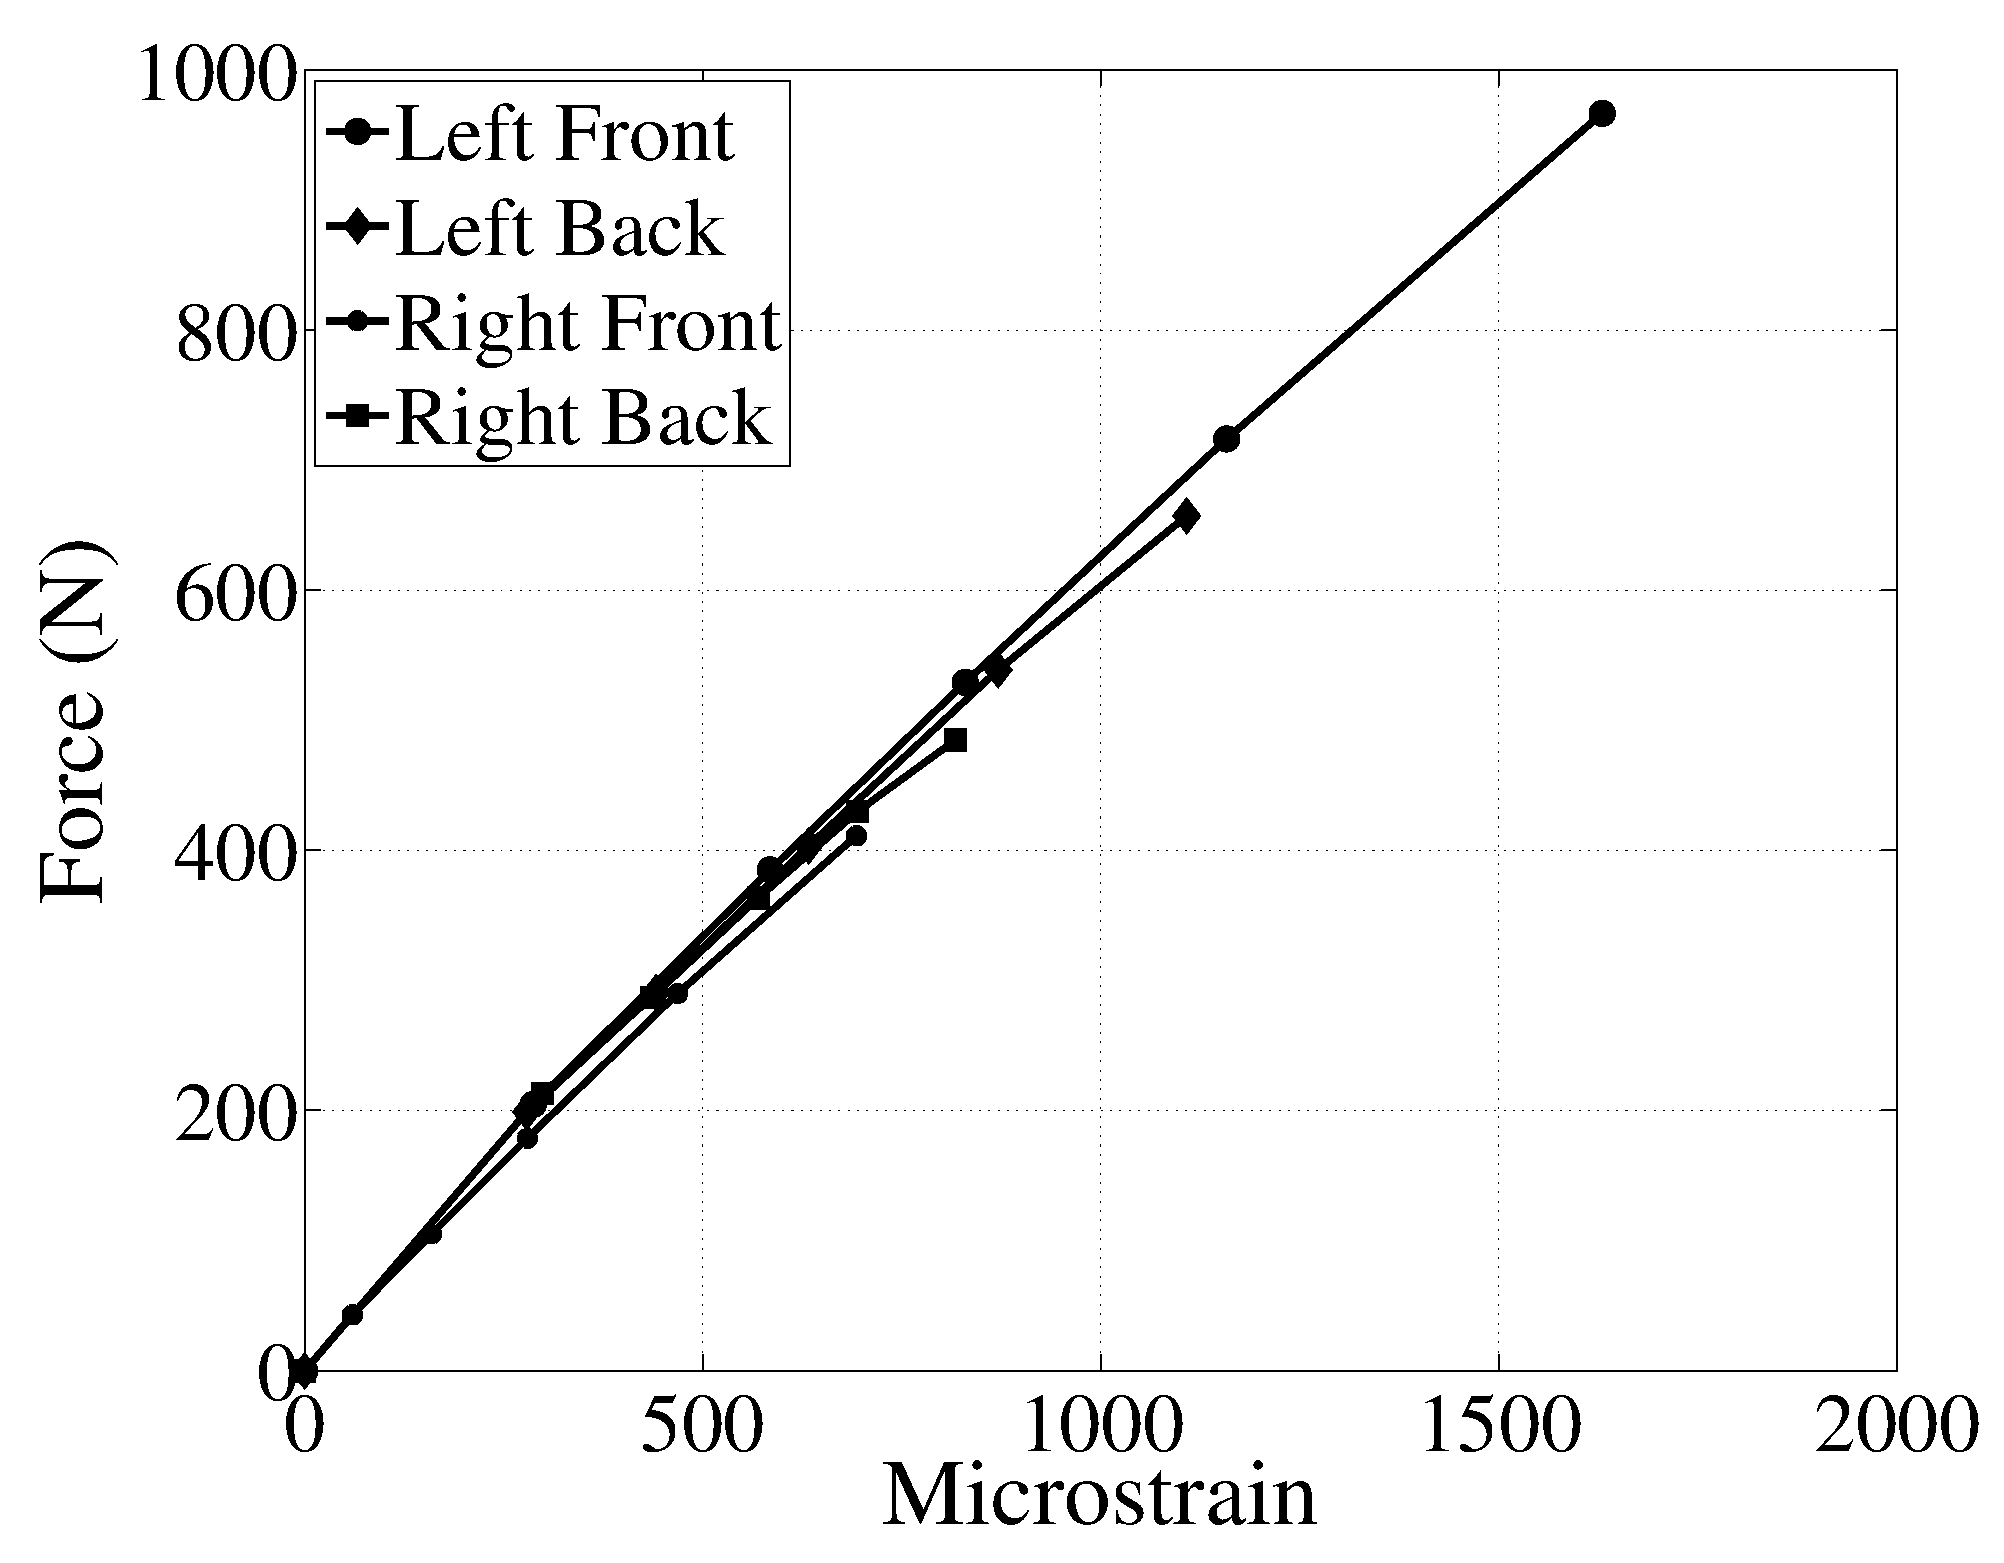
\includegraphics[width=0.7\linewidth]{./appendixDvc/figures/CrossLoadCalibration}
\caption[\acs*{dvc} cross load device calibration]{\textbf{Calibration curves for the \acs*{dvc} cross load calibration device. Every post has approximately the same calibration value.} Graphic \copyright Seth Gilchrist, 2013.}
\label{fig:CrossLoadCalibration}
\end{figure}

\clearpage

\section{Verification of \acs*{dvc}}
\label{sec:dvc_results_validation}
The \ac{dvc} algorithm was tested in two ways.
First a verification of the algorithm was conducted by synthetically warping an image and then using the \ac{dvc} algorithm to calculate the known, ground truth strain.
The second was a validation of the \ac{hrpqct} in which a bone was scanned twice in the same position under no load and the \ac{dvc} algorithm was used to measure the strain, which should result in a uniform value of zero strain.

\subsection{Synthetically strained image}
\label{sec:dvc_results_synthetic}
The \ac{dvc} algorithm was characterized using synthetically strained images.
A \ac{ct} image of a bone sample was deformed using a quadratic deformation, resulting in a linearly increasing strain across the image.

\acused{dicom}
A single human femoral bone specimen was scanned in the \ac{chhm} \ac{hrpqct} (XtremeCT, Scanco, Br\"{u}ttisellen, Switzerland) at an isotropic resolution of 0.041~\ac{mm}.
Following scanning, a section of cancellous bone was isolated and exported to \ac{dicom} format.
The \ac{dicom} images were read using \ac{itk} and synthetically strained using a quadratic deformation, resulting in a linearly increasing strain (Figure~\ref{fig:CompareStrain5Percent}).
The code used to preform the deformation can be found with the other \ac{dvc} code in \S\ref{sec:code_dvc}.
Two strain fields were investigated.
In the first, strain varied linearly from 0 to -1\% strain and in the second, the strain varied linearly from 0 to -5\% strain.

\begin{figure}
\centering
\includegraphics[width=.8\linewidth]{./appendixDvc/figures/CompareStrain5Percent}
\caption[5\% synthetic strain comparison]{\textbf{The linear strain to 5\% maximum is shown. The bone image (far left) that was deformed using a quadratic field to produce a linearly increasing strain from 0 to -5\% (middle left). The \ac{dvc} algorithm was used to measure the strain (far right) and the difference between the true strain and the measuered strain could be evaluated (middle right).} Image \copyright Seth Gilchrist, 2013.}
\label{fig:CompareStrain5Percent}
\end{figure}

The strain measured by the \ac{dvc} algorithm tracked the applied strain closely (Figure~\ref{fig:SyntheticStrain}).
Analysis of the~0 to~-1\% image had low strain errors, with an average difference from the applied strain of 0.0047\% strain.
Analysis of the~0 to~-5\% image had larger error magnitudes, but the average error was still low (0.057\%).
Both of these errors are below cancellous bone yield strain (Table~\ref{tab:bone_fail}).

\begin{figure}
\centering
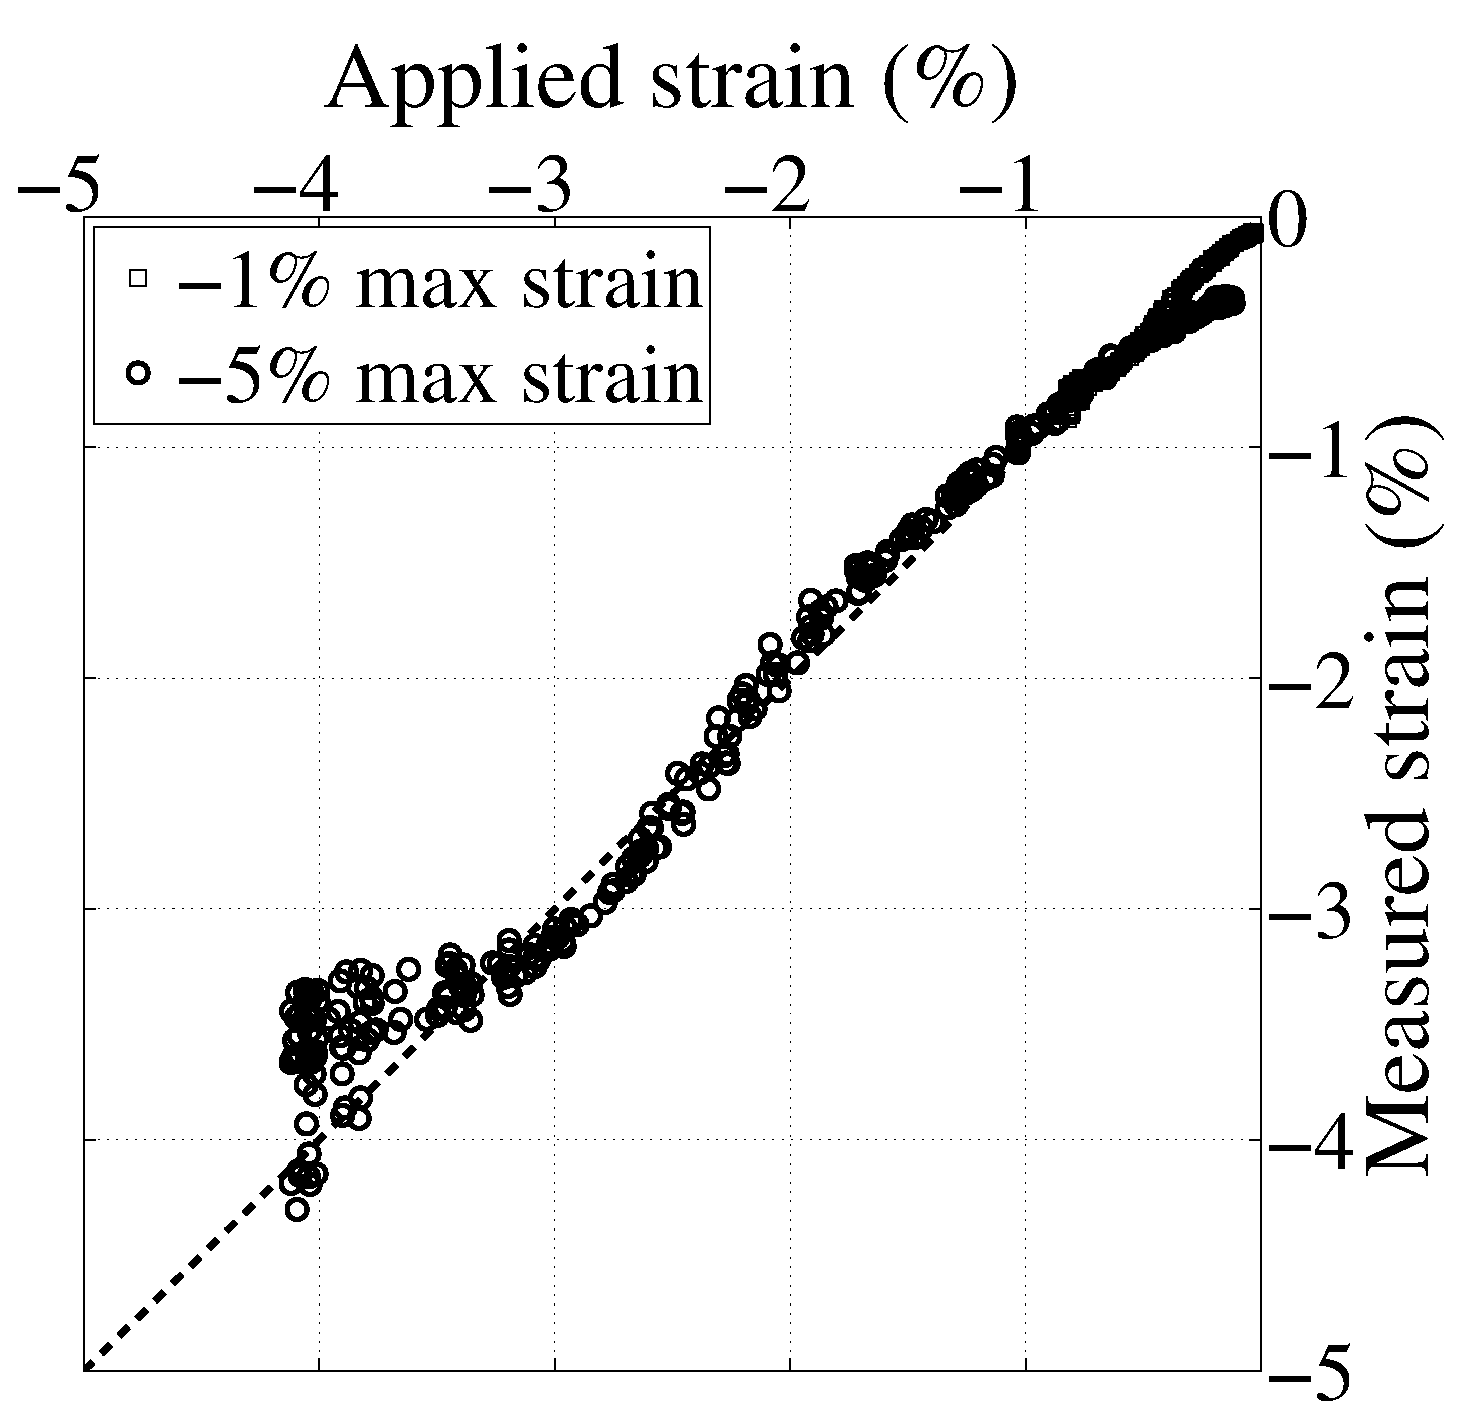
\includegraphics[width=0.7\linewidth]{./appendixDvc/figures/SyntheticStrain}
\caption[Synthetic strain results]{\textbf{The compiled results of the synthetic strain test. Two tests are shown here, one with linearly increasing strain from~0 to~-1\% ($DVC = 1.024 \cdot actual+0.015$, $R^2 = .988$) and a separate test with linearly increasing strain from~0 to~-5\% ($DVC = 1.081 \cdot actual+0.113$, $R^2 = .979$).} Graphic \copyright Seth Gilchrist, 2013.}
\label{fig:SyntheticStrain}
\end{figure}

Both the~-1\% and~-5\% tests showed a sensitivity high enough to detect strains below yield strain in cancellous bone.
The~-5\% tests showed less agreement than the~-1\% test in the region of overlap, and it is thought that this might be due to the higher strain gradient present in the~-5\% results.
The affine transform used by the \ac{dvc} is linear in nature and would under represent the shape functions required to capture the quadratic deformation used to create the linearly increasing strain.
Additionally, the quality of the results decreased at compressive strains of grater than~-3\%.
This could be due to decreased region size in the end of the measurement volume.
The \ac{dvc} algorithm selects a subregion with dimensions set by the user (determined by the \ac{tbsp}), however, if the desired region is outside of the image, the subregion will be clipped by the image bounds.
This reduction in subregion size at the edges of a measurement volume could affect the accuracy of any strain measurements near the edge of the image in a systematic way.
It is therefore recommended that analyses be conducted in images that are much larger than the measurement region.

\subsection{Zero strain image}
\label{sec:dvc_results_zero}
In this experiment a single human proximal femur was scanned in the \ac{hrpqct} using the same protocol as in \S\ref{sec:dvc_results_synthetic}.
Instead of taking a single image, two images were take in succession.
Overlapping regions of the two images were extracted and saved in \ac{dicom} format and analysed using the \ac{dvc} algorithm.

\ac{dvc} of the two image should show no strain, however, the results showed a band of non-zero strain running through the middle of the measurement volume (Figure~\ref{fig:ZeroStrain}).
The majority of the measurement volume showed low strain values (Figure~\ref{fig:ZeroStrainHist}).
The bimodal distribution seen in the histogram displays that the majority of the measurement volume enjoyed low error values (median of strains \textless 0.25\% = 0.12\%).
The central band of high strain created a second, normally distributed peak, with an value of (average (\ac{sd})) 0.45(.07\%).

\begin{figure}
\centering
\includegraphics[width=0.8\linewidth]{./appendixDvc/figures/ZeroStrain}
\caption[Zero strain results]{\textbf{Two images were taken in succession with no applied strain between them. The resulting \acs*{dvc} analysis showed a band of non-zero strain that was located at a junction of two \acs*{hrpqct} slice blocks. Misalignment of the slice blocks in the reconstruction of the \ac{ct} data resulted in a 0.5~voxel discontinuity in the image, creating the linear strain shown. The image shows the analysis region, rendered transparently, with contours of constant compressive strain greater than -0.15\%.} Graphic \copyright Seth Gilchrist, 2013}
\label{fig:ZeroStrain}
\end{figure}

\begin{figure}
\centering
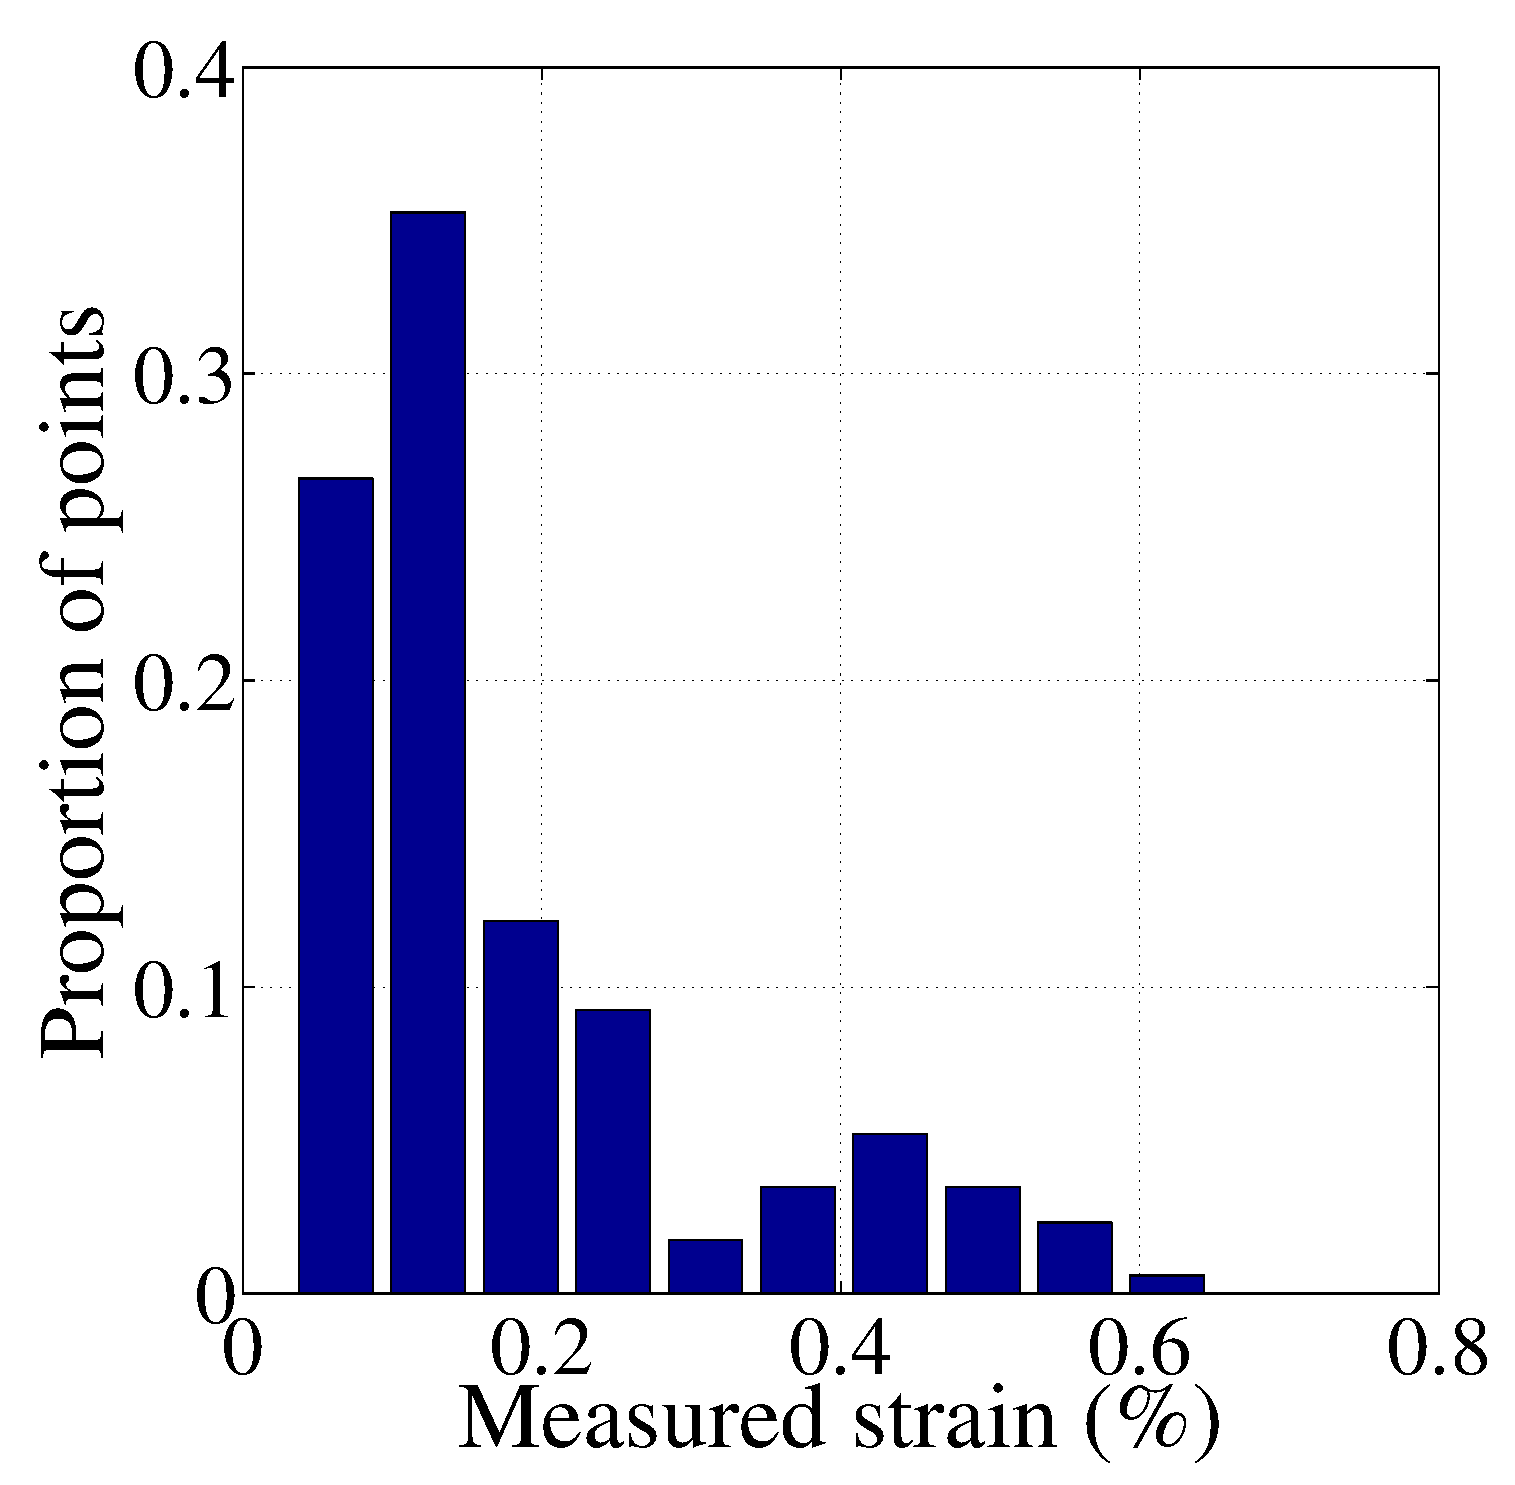
\includegraphics[width=0.7\linewidth]{./appendixDvc/figures/ZeroStrainHist}
\caption[Zero strain histogram]{\textbf{Results histogram for the zero strain measurement. The results show a bimodial distribution, with the majority of the volume having an error of approximately 0.12\%, and a small number of centrally located voxels having an error of 0.45\% strain.} Graphic \copyright Seth Gilchrist, 2013.}
\label{fig:ZeroStrainHist}
\end{figure}

The central band of high strain was seen to be on the junction of two \ac{hrpqct} slice blocks.
The XtremeCT takes images in blocks of 220~slices when acquiring at 0.041~\ac{mm} resolution.
The blocks of slices are axially registered together during reconstruction using data from the machine stepper motors, which have a finite accuracy.
While the accuracy varies, this junction displayed an approximately 0.5~voxel discontinuity, resulting in the elevates stains across it.
Indeed, only one of the two images used for this analysis showed evidence of a slice block discontinuity, and other slice block junctions in the same volume did not show such an artefact.
The erroneous strains are not limited to the slice block junction for two reasons.
First, the mesh nodes are nominally spaced in this analysis by 2~\ac{mm}, so the discontinuity was between two registration subregion centres, increasing the strain for the \ac{fe} element defined by the nodes at the centres of the subregions.
Secondly, the subregions used for analysis were 2.67~\ac{mm} on a side, so measurement locations that were up to 1.3~\ac{mm} away from the image discontinuity could have been affected.

The results of this analysis indicate that the \ac{hrpqct} image acquisition protocol lacks the accuracy to be able to acquire images needed for \ac{dvc} reliably.
However, the errors noted here are not pervasive, and certain analyses could be performed as long as the acquired images are cleared of slice block discontinuities.

\section{\acs*{dvc} experimental results}
\label{sec:dvc_results_exp}
Two experiments have been conducted using the \ac{dvc} algorithm.
One experiment used the axial loading apparatus to apply compressive forces to a mouse vertebral body.
The second used image data from compression of a bone in a high resolution microCT.
The methods and results are detailed here, along with a discussion about the utility and effectiveness of the \ac{dvc} algorithm.

\subsection{Axial compression of a rabbit vertebra}
\label{sec:dvc_results_rabbit}\acused{c}
A single, fresh frozen vertebra from a New Zealand white rabbit (female, 5~months) was obtained in conjunction with an ongoing study at the \ac{ubc}.
The bone was excised and stored in saline soaked cloth at -20$^\circ$~\ac{c} until the current study began.
It was thawed to room temperature overnight and soft tissues and processes were removed.
The bone was potted in \ac{pmma} (\acs{pmma}, Bosworth Co, Skokie, IL) using the potting device descried in~\S\ref{sec:dvc_apparatus_axial} (Figure~\ref{fig:vertebraPretest}).
Axial loads were applied using the axial loading device detailed in \S\ref{sec:dvc_apparatus_axial}.
Force was applied in 180~\ac{n} increments, and the bone was allowed to relax for 15~\acs{min} after loading.
The bone was then scanned in an \ac{hrpqct} (XtremeCT, Scanco, Br\"{u}ttisellen, Switzerland) at an isotropic resolution of 0.041~\ac{mm}.

\begin{figure}
\centering
\includegraphics[width=0.7\linewidth]{./appendixDvc/figures/vertebraPretest}
\caption[Rabbit vertebra before testing]{\textbf{The rabbit vertebra in the \acs*{pmma} potting before testing. The callipers are open 1~\ac{cm} for scale.} Graphic \copyright Seth Gilchrist, 2013.}
\label{fig:vertebraPretest}
\end{figure}

The bone was segmented from the surroundings using 3DSlicer (3.0, 3DSlicer, \url{http://www.slicer.org/}) and a saved as a \ac{stl} file.
The \ac{stl} file was imported into Gmsh (2.8, Gmsh, \url{http://geuz.org/gmsh/}) and a \ac{3d}, linear tetrahedral mesh with node spacing of 1.6~\ac{mm} was created.
Results were visualized in Paraview (3.98, Paraview, \url{http://paraview.org/}).

The rabbit vertebra failed between 540~\ac{n} and 720~\ac{n}.
The strain in the vertebra increased steadily as loads were increased, with the highest strains being measured in the end plates (Figure~\ref{fig:Comparison3}).
The strain in the caudal end plate averaged~10.1\% at~540~\ac{n}.
The cranial end plate also showed high strain, but not to the same degree as the caudal one.
The specimen fractured in the transverse plane, in what appeared to be a bending mode, in a location of purely cortical bone (Figure~\ref{fig:vertebraPostTest}).

\begin{figure}
\centering
\includegraphics[width=\linewidth]{./appendixDvc/figures/Comparison3}
\caption[Rabbit vertebra compression]{\textbf{The compressed rabbit vertebra showed increasing strain as force increased. The highest strain was seen in the caudal end plate.} Graphic \copyright Seth Gilchrist, 2013.}
\label{fig:Comparison3}
\end{figure}

\begin{figure}
\centering
\includegraphics[width=.8\linewidth]{./appendixDvc/figures/vertebraPostTest}
\caption[Rabbit vertebra after testing]{\textbf{The rabbit vertebra failed in the transverse plane in what appeared to be a bending mode, in predominantly cortical bone. The callipers are open 1~\ac{cm}.} Graphic \copyright Seth Gilchrist, 2013.}
\label{fig:vertebraPostTest}
\end{figure}

Extreme strains were measured by the \ac{dvc} algorithm in the end plate region of the rabbit vertebra.
These strain levels were above failure strain for cancellous bone, however, in this specimen the strains appear to be accurate when compared to a \ac{2d} approximation obtained from examination of the slice data shown in Figure~\ref{fig:RawImagesTogether}.
New Zealand white rabbits do not reach skeletal maturity until an age of 7--9~months~\citep{masoud_longitudinal_1986}, meaning that the end plates in the 4~month old vertebra used in this experiment would not have fused yet.
Direct observation of the \ac{ct} images showed that the strain was developed by the collapse of a growth plate and the subsequent compression of the soft bone at in the reserve, proliferating and hypertrophic growth plate zones (Figure~\ref{fig:RawImagesTogether}).

\begin{figure}
\centering
\includegraphics[width=.7\linewidth]{./appendixDvc/figures/RawImagesTogether}
\caption[Rabbit vertebra growth plate]{\textbf{High strains were developed in the growth plate (red arrows) of the rabbit vertebra. The plate collapsed and then compression of the soft bone allowed for increased strain.} Graphic \copyright Seth Gilchrist, 2013.}
\label{fig:RawImagesTogether}
\end{figure}

The \ac{dvc} algorithm also detected high strains in the central portion of the bone, in a region that was predominantly cortical bone.
The algorithm isn't sensitive to deformations of cortical bone because the images lack texture for tracking in the cortical bone at the 0.041~\ac{mm} resolution.
Examination of the displacement field showed an erroneous vector in the region of this high strain that was approximately 2.8x the average displacement in the rest of the bone.
This single displacement vector was responsible for the region of high strain, and it could be discounted based on its identification.

This tests shows the utility of the \ac{dvc} algorithm for investigating the internal strain fields of bones loaded under compressive forces.
It identified and quantified the strain in the collapse of the growth plate, which was not anticipated.
This demonstrates the ability of the \ac{dvc} algorithm to act as an independent tool, uninformed about anticipated material properties, for measurement of deformation phenomena.

\subsection{Axial compression of a human bone core}
\label{sec:dvc_results_human}
For this experiment, x-ray data were obtained from another lab (Dr.~Michael Liebschnre, Baylor Collage of Medicine, Houston, TX) which had performed axial compression of human cancellous bone in a microCT machine at an isotropic resolution of 0.018~\ac{mm}.
The bone was imaged first in an uncompressed state, and then successively imaged at increasing levels of compression.
No information was available on the displacement or load levels for each compression.

The specimens were cylindrical, 10~\ac{mm} tall and 8~\ac{mm} in diameter.
They were loaded axially along their longest dimension.
Because the specimens were of simple geometry, no segmentation was required.
A cylinder was constructed in Gmsh (2.8, Gmsh, \url{http://geuz.org/gmsh/}) and meshed using linear, tetrahedral elements, with an node spacing of 2.8~\ac{mm}.
The \ac{dvc} was conducted using square subregions, 3.6~\ac{mm} on a side.

The analysis showed a linear deformation with increasing strains in the top of the cylinder with each successive compression (Figure~\ref{fig:CompareSteps1-4WithBone}).
Additional steps were available, however the \ac{dvc} began to produce erratic results when the strain magnitudes were above 20\%.
The calculated nominal strain at step four was 5.7\%, with a maximum local strain on the top, side of the cylinder of 22\% strain.
The average displacement in the first loading step was 0.05~\ac{mm}, with a calculated range of 0.030--0.099~\ac{mm}.

\begin{figure}
\centering
\includegraphics[width=\linewidth]{./appendixDvc/figures/CompareSteps1-4WithBone}
\caption[Human bone compression]{\textbf{The human bone did not compress uniformly, but showed high compression near the moving platen, and lower compression at the bottom support. In this graphic, the mesh has been deformed by the measured displacement.} Graphic \copyright Seth Gilchrist, 2013.}
\label{fig:CompareSteps1-4WithBone}
\end{figure}

The increased strain on the side of the cylinder was observed from the first loading step (not visible in Figure~\ref{fig:CompareSteps1-4WithBone} due to the large colour bar range.), indicating that the specimen was likely either not aligned perfectly to the loading direction or the ends were not milled completely parallel.
This was corroborated by the range of measured displacements in the first loading step.
The specimen continued to exhibit high strain in the one location, which indicates that the specimen was probably slightly taller in that location, leading to increased strain.
Additionally, examination of the bone image in Figure~\ref{fig:CompareSteps1-4WithBone} showed that the location of high strain had fewer trabeculi, indicating that this location may have been be weaker, and possibly prone to strain localization before failure of the opposite side.
Indeed as the overall compression increased, we saw a more equitable distribution of the strain in the top of the specimen.
If the analysis had continued, it would have been possible to examine the strain relaxation after failure.

High strains in the specimen at steps five and greater lead to erratic strain results.
It is possible that this could have been prevented through the use of differential analysis.
In the steps up to step four, the deformed bone specimen was compared directly to the undeformed specimen.
However, at higher deformations the shape functions provided by the affine transform were not sufficient, and the radius of convergence of even the regular step gradient descent optimizer was not large enough to identify the subregion in the original image.
A differential analysis would compare the image at step five with the image at step four using the step~4's results as an initial guess of the solution, and potentially improving the results.
This technique is, however, not ideal for \ac{dvc} because measurement errors in the comparison of, e.g., steps~4 and~5, would be transferred into the measurement of steps~5 and~6, and a general accumulation of error would result.
At the time of this experiment, the \ac{dvc} algorithm did not have this capabiliyt.
However, it has since been added in the form of a ``restart" mesh, \ac{ie}, a mesh file that is already populated with deformation data at each node which acts as the starting point for the next registration.
While the ability to perform differential \ac{dvc} has been incorporated, it has not been tested.

This experiment displayed the \ac{dvc} algorithm's capability to examine the detailed deformation and strain development in bone samples.
The identification of a presumed edge loading phenomenon displays the utility of this method as a \acf{fe} validation.
The displacement outputs of the \ac{dvc} algorithm could be used as boundary conditions for an \ac{fe} analysis, and the resulting strain fields compared.
Identification of edge loading, as seen here, would be nearly impossible using typical axial compression techniques.
Small changes in the boundary conditions can have a profound influence on the \ac{fe} calculated strains and independent measures of such as this could have a positive influence on calculation accuracy.

\section{\acs*{dvc} discussion}
\label{sec:dvc_discussion}
The \acl{dvc} algorithm presented in this appendix has was developed with the intent that it could be used to assist in the validation of \ac{fe} analysis results.
The algorithm was developed using state of the art, open source image registration techniques, optimized based on the particular requirements of the application.
It has been shown to be capable of measuring strains that are well below yield strains of cancellous bone in synthetically deformed images.
It is also capable of detecting small strains in human and animal bones, without the need for a priori knowledge of potential deformations or reliance on precise boundary conditions.

Even though these advantages are important, it is also important to note the limitations of the technique.
The \ac{dvc} algorithm is itself a computational technique that cannot be taken as a ground truth solution.
A next step would be to use the technique in conjunction with \acl{fe} analysis, or more traditional \acl{dic} and use a mutual validation method such as proposed by \citet{bland_statistical_1986}.
Practically, the algorithm has shown issues with measuring extremely high strains, particularly those over 20\% in the case of a compressively loaded human bone, and above 4\% in a synthetically deformed human bone image.
The latter was more likely an issue measuring the quadratic displacement field than with the ability of the algorithm, per se.
The application of the algorithm to measurements taken in the XtremeCT, \ac{hrpqct} scanner also showed the potential for large measurement errors due to aspects of how the \ac{ct} machine performs its reconstructions.
While these problems were not pervasive in nature, they have the ability to hamper the use of \ac{dvc} in larger specimens.
An improved scanning technique, in which slice blocks are acquired with overlap and then registered using image, rather than stepper motor, data has been proposed and is in early stages of testing.
If successful, this technique could make the use of \ac{dvc} reliable in the \ac{hrpqct}.

Overall, the \ac{dvc} technique and its current manifestation presented in this document and detailed in the code given in~\S\ref{sec:code_dvc} show a high degree of promise.
While it is still a research tool that requires an knowledgeable user, the possibility to inform and validate \ac{fe} analyses using the algorithm makes it a worthwhile tool for continued exploration.